\begin{figure*}[t]
\providecommand{\width}{}
\renewcommand{\width}{0.18\textwidth}
\centering
\begin{subfigure}[t]{\width}

\includegraphics[width=\textwidth]{figures/tasks/cup}
\caption{Cup}
\end{subfigure}\hfill%
\begin{subfigure}[t]{\width}
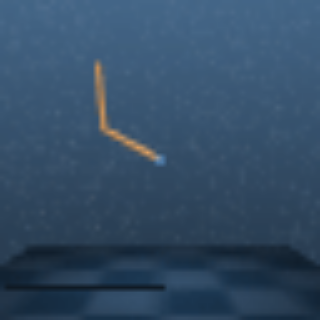
\includegraphics[width=\textwidth]{figures/tasks/acrobot}
\caption{Acrobot}
\end{subfigure}\hfill%
\begin{subfigure}[t]{\width}
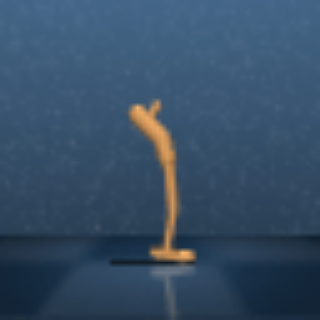
\includegraphics[width=\textwidth]{figures/tasks/hopper}
\caption{Hopper}
\end{subfigure}\hfill%
\begin{subfigure}[t]{\width}

\includegraphics[width=\textwidth]{figures/tasks/walker}
\caption{Walker}
\end{subfigure}\hfill%
\begin{subfigure}[t]{\width}
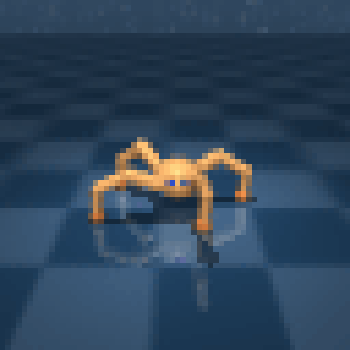
\includegraphics[width=\textwidth]{figures/tasks/quadruped}
\caption{Quadruped}
\end{subfigure}\hfill%
\caption{Image observations for 5 of the 20 visual control tasks used in our experiments. The tasks pose a variety of challenges including contact dynamics, sparse rewards, many degrees of freedom, and 3D environments. Several of these tasks could previously not be solved through world models.}
\label{fig:tasks}
\vspace*{-1ex}
\end{figure*}